\documentclass{beamer}
%\usecolortheme[named=green]{structure}
\mode<presentation> {
\usetheme{CambridgeUS}
\usecolortheme{orchid}
\usefonttheme{structuresmallcapsserif}
%\setbeamercovered{invisible}
% To remove the navigation symbols from the bottom of slides%
\setbeamertemplate{navigation symbols}{} 
}
 \setbeamertemplate{footline}
        {
      \leavevmode
      \hbox{
      \begin{beamercolorbox}[wd=.36\paperwidth,ht=2.25ex,dp=1ex,center]{author in head/foot}
        \usebeamerfont{author in head/foot}\insertshortauthor~~(\insertshortinstitute)
      \end{beamercolorbox}
      \begin{beamercolorbox}[wd=.56\paperwidth,ht=2.25ex,dp=1ex,center]{title in head/foot}
        \usebeamerfont{title in head/foot}\insertshorttitle
      \end{beamercolorbox}
      \begin{beamercolorbox}[wd=.08\paperwidth,ht=2.25ex,dp=1ex,right]{date in head/foot}
        \usebeamerfont{date in head/foot}\insertframenumber{}\hspace*{2em}

      \end{beamercolorbox}}
      \vskip0pt
    }

\usepackage{graphicx}
\title[ Schedule C Appointments]{Schedule C Appointments}
%
\author{Emily Moore}
\institute[WUSTL]
{
Washington University-St. Louis \\
\medskip
{\emph{emily.moore@wustl.edu}}
}
\date{\today}
% \today will show current date. 
% Alternatively, you can specify a date.

\usepackage{Sweave}
\begin{document}
\Sconcordance{concordance:PresentationApr22.tex:PresentationApr22.Rnw:%
1 41 1 1 0 179 1}


\begin{frame}
\titlepage
\end{frame}

\begin{frame}
\frametitle{Project Recap}
\begin{itemize} \addtolength{\itemsep}{1\baselineskip}
\item Schedule C appointments: Appointments of a confidential or policy-determining nature not subject to competitive hiring or advice and consent.
\item Original paper looked at this through lens of presidential attention...
\item ...But probably the president isn't doing the hiring...
\item ...and people have had concerns about patronage.
\end{itemize}
\end{frame}

\begin{frame}
\centering
\begin{figure}
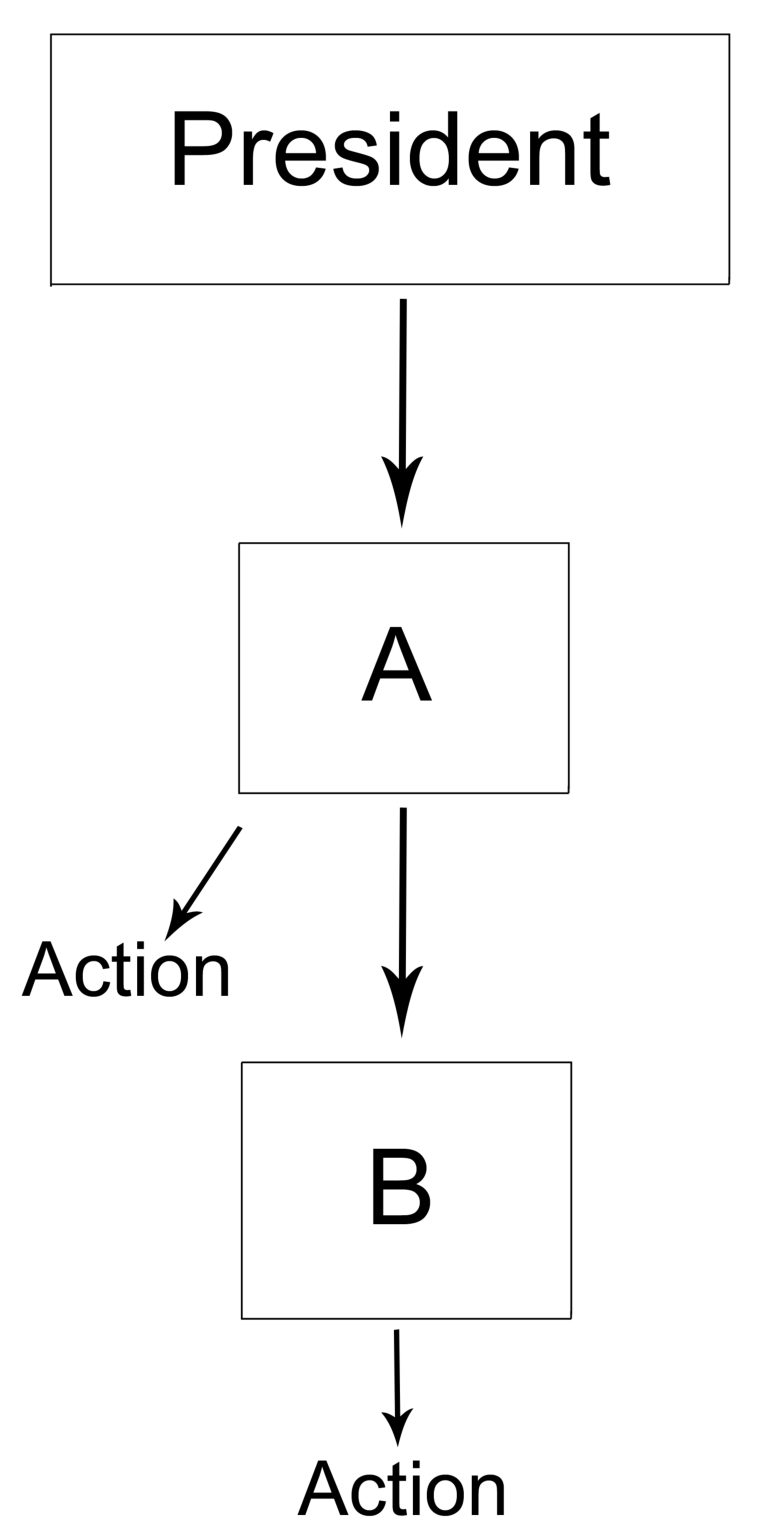
\includegraphics[height=3.25in,width=1.5in]{ModelV1.pdf}
\end{figure}
\end{frame}

\begin{frame}
\centering
\begin{figure}
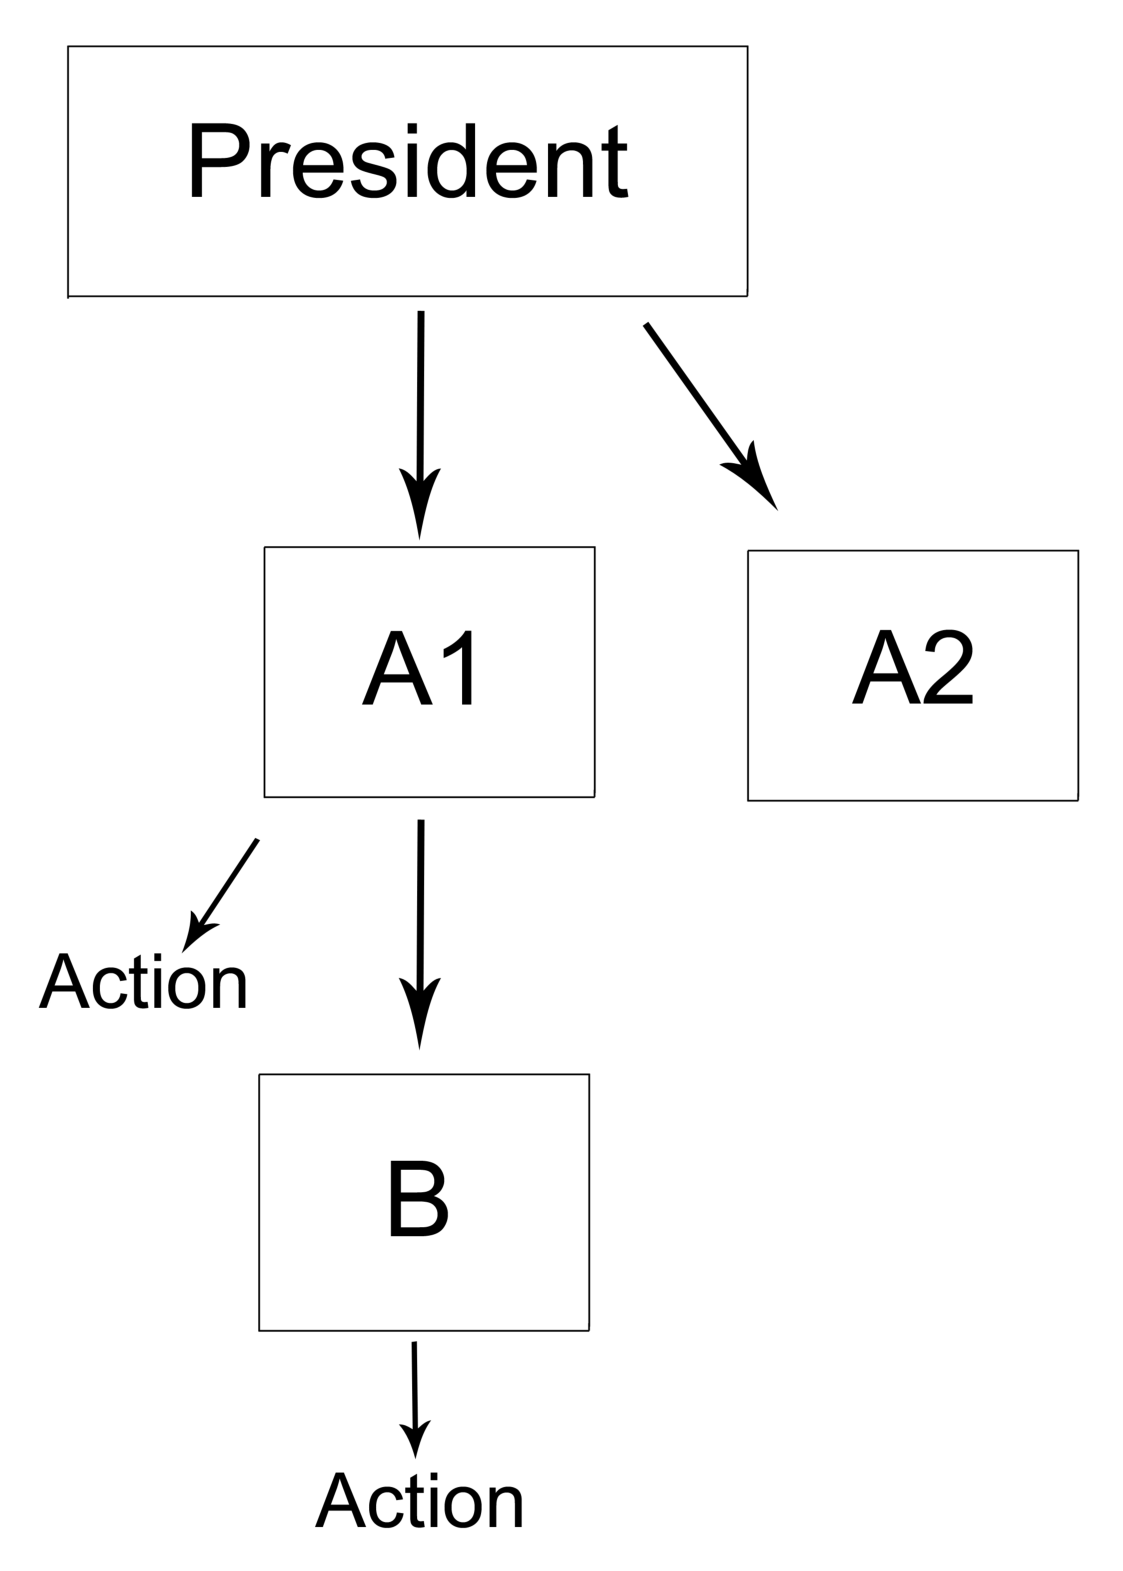
\includegraphics[height=3.4in,width=2.3in]{ModelV2.pdf}
\end{figure}
\end{frame}

\begin{frame}
\centering
\begin{figure}
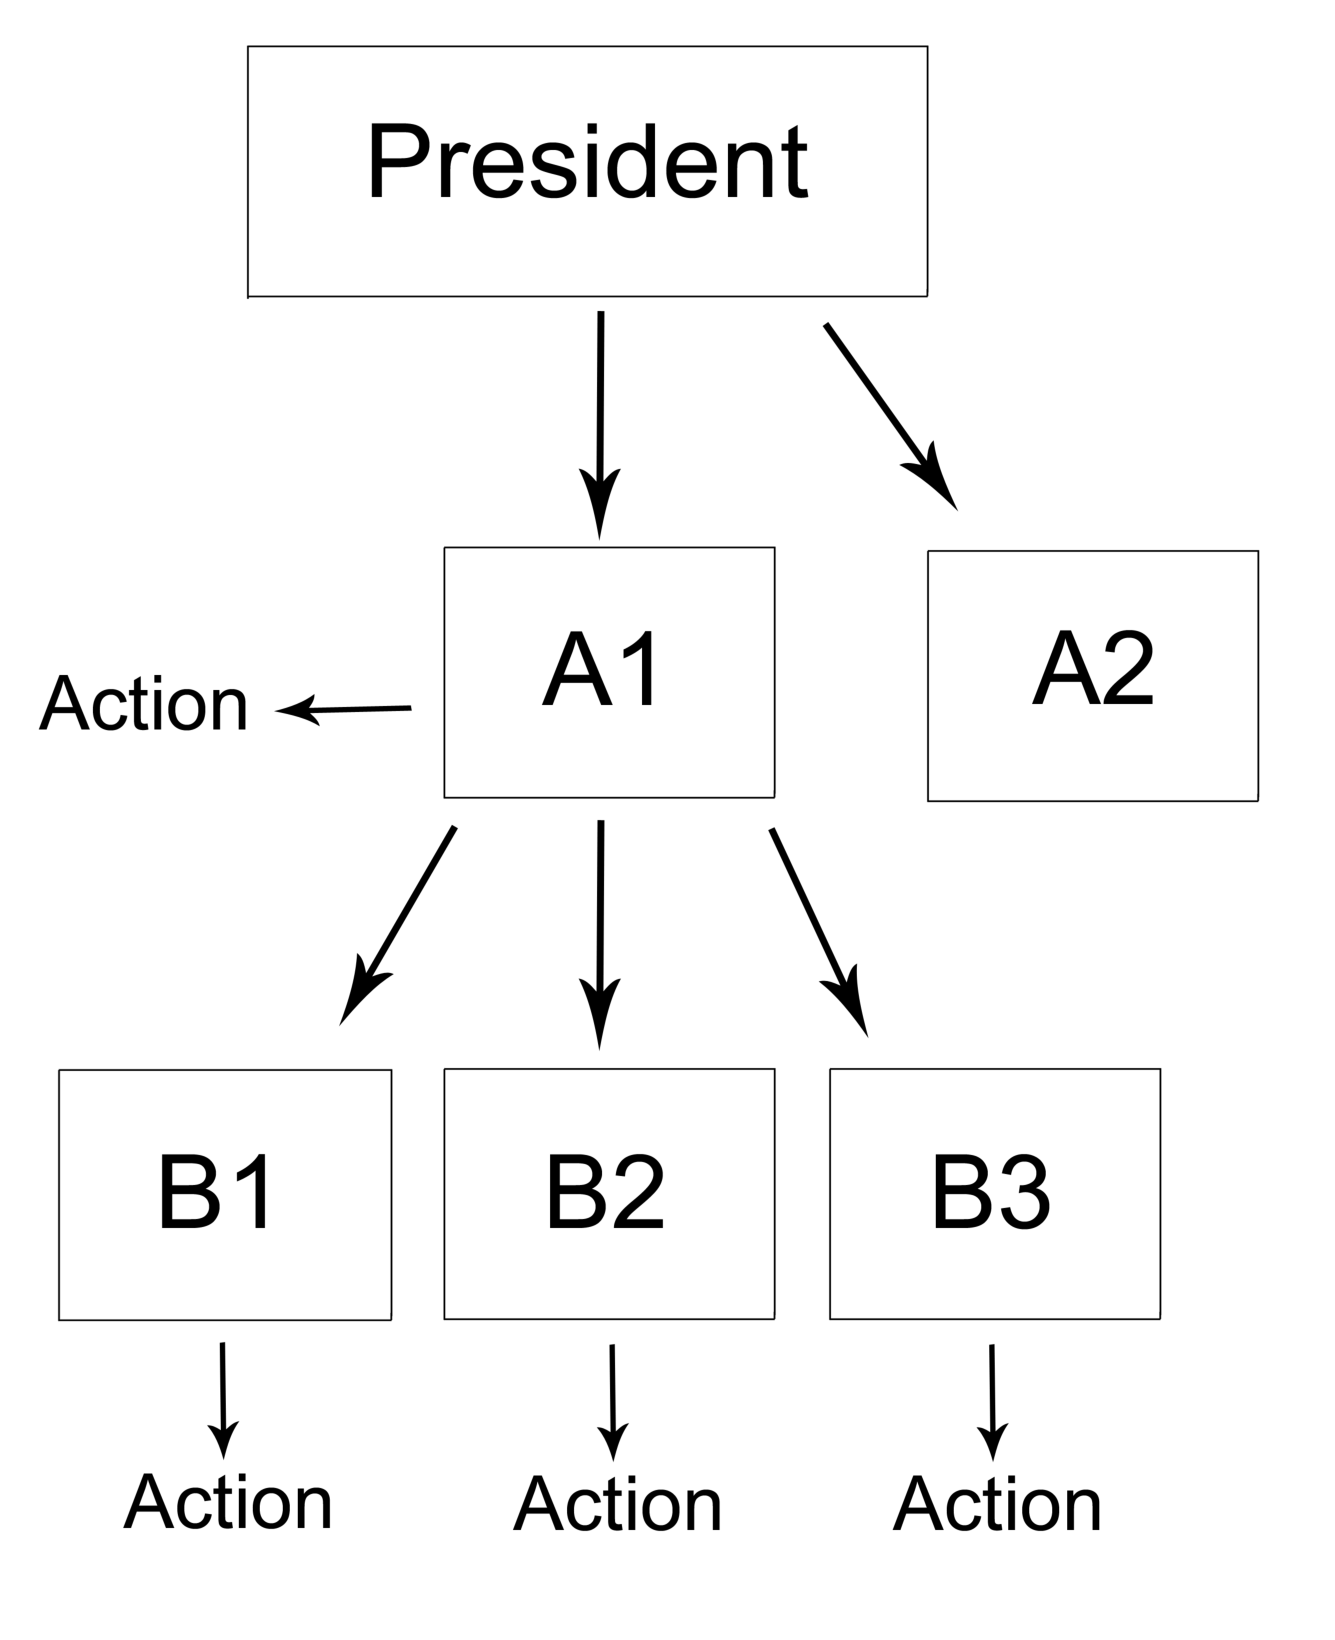
\includegraphics[height=3.25in,width=2.5in]{ModelV3.pdf}
\end{figure}
\end{frame}

\begin{frame}
\frametitle{The Data}
\begin{itemize} \addtolength{\itemsep}{1\baselineskip}
\item Count Data from Federal Register
\item Observe A picking B
\item Observe A's Actions
\item Observe B's Actions???
\end{itemize}
\end{frame}

\begin{frame}[fragile]
\frametitle{Example XML entries from Federal Register}
\footnotesize
\begin{verbatim}
<HD SOURCE="HD2">Department of State</HD>
<FP SOURCE="FP-1">DSGS69951Staff Assistant to the Special Envoy with the Rank of Ambassador. Effective November 30, 2009.</FP>
<FP SOURCE="FP-1">DSGS69975Special Assistant to the Secretary of State. Effective November 30, 2009.</FP>

<HD SOURCE="HD2">Department of the Treasury</HD>
<FP SOURCE="FP-1">DYGS60390Senior Advisor to the Assistant Secretary and Chief Financial Officer. Effective November 24, 2009.</FP>

<HD SOURCE="HD2">Department of Defense</HD>
<FP SOURCE="FP-1">DDGS17262Special Assistant to the Director, Operational Test and Evaluation. Effective November 06, 2009.</FP>

<FP SOURCE="FP-1">DDGS17265Deputy White House Liaison to the Special Assistant for White House Liaison. Effective November 09, 2009.</FP>
<FP SOURCE="FP-1">DDGS17264Special Assistant to the Principal Deputy Assistant Secretary of Defense for Legislative Affairs. Effective November 20, 2009.</FP>
<FP SOURCE="FP-1">DDGS17266Special Assistant to the Deputy Assistant Secretary of Defense for Cyber and Space Policy. Effective November 20, 2009.</FP>

<HD SOURCE="HD2">Department of Homeland Security</HD>
<FP SOURCE="FP-1">DMGS00817Special Assistant to the Officer of Civil Rights and Civil Liberties. Effective November 13, 2009.</FP>

<HD SOURCE="HD2">Department of the Interior</HD>
<FP SOURCE="FP-1">DIGS01175Deputy Director to the Director, Congressional and Legislative Affairs. Effective November 20, 2009.</FP>
\end{verbatim}
\end{frame}

\begin{frame}[fragile]
\frametitle{Example XML entries from Federal Register}
\scriptsize
\begin{verbatim}
Department of State
DSGS69951Staff Assistant to the Special Envoy with the Rank of Ambassador. 
Effective November 30, 2009.

DSGS69975Special Assistant to the Secretary of State. 
Effective November 30, 2009.

Department of the Treasury
DYGS60390Senior Advisor to the Assistant Secretary and Chief Financial Officer. 
Effective November 24, 2009.

Department of Defense
DDGS17262Special Assistant to the Director, Operational Test and Evaluation. 
Effective November 06, 2009.

DDGS17265Deputy White House Liaison to the Special Assistant 
for White House Liaison. 
Effective November 09, 2009.

DDGS17264Special Assistant to the Principal Deputy Assistant Secretary of 
Defense for Legislative Affairs. 
Effective November 20, 2009.

DDGS17266Special Assistant to the Deputy Assistant Secretary of Defense 
for Cyber and Space Policy. 
Effective November 20, 2009.

Department of Homeland Security
DMGS00817Special Assistant to the Officer of Civil Rights and Civil Liberties. 
Effective November 13, 2009.

Department of the Interior
DIGS01175Deputy Director to the Director, Congressional and Legislative Affairs. 
Effective November 20, 2009.
\end{verbatim}
\end{frame}

\begin{frame}[fragile]
\frametitle{Example day from Federal Register}
\begin{figure}
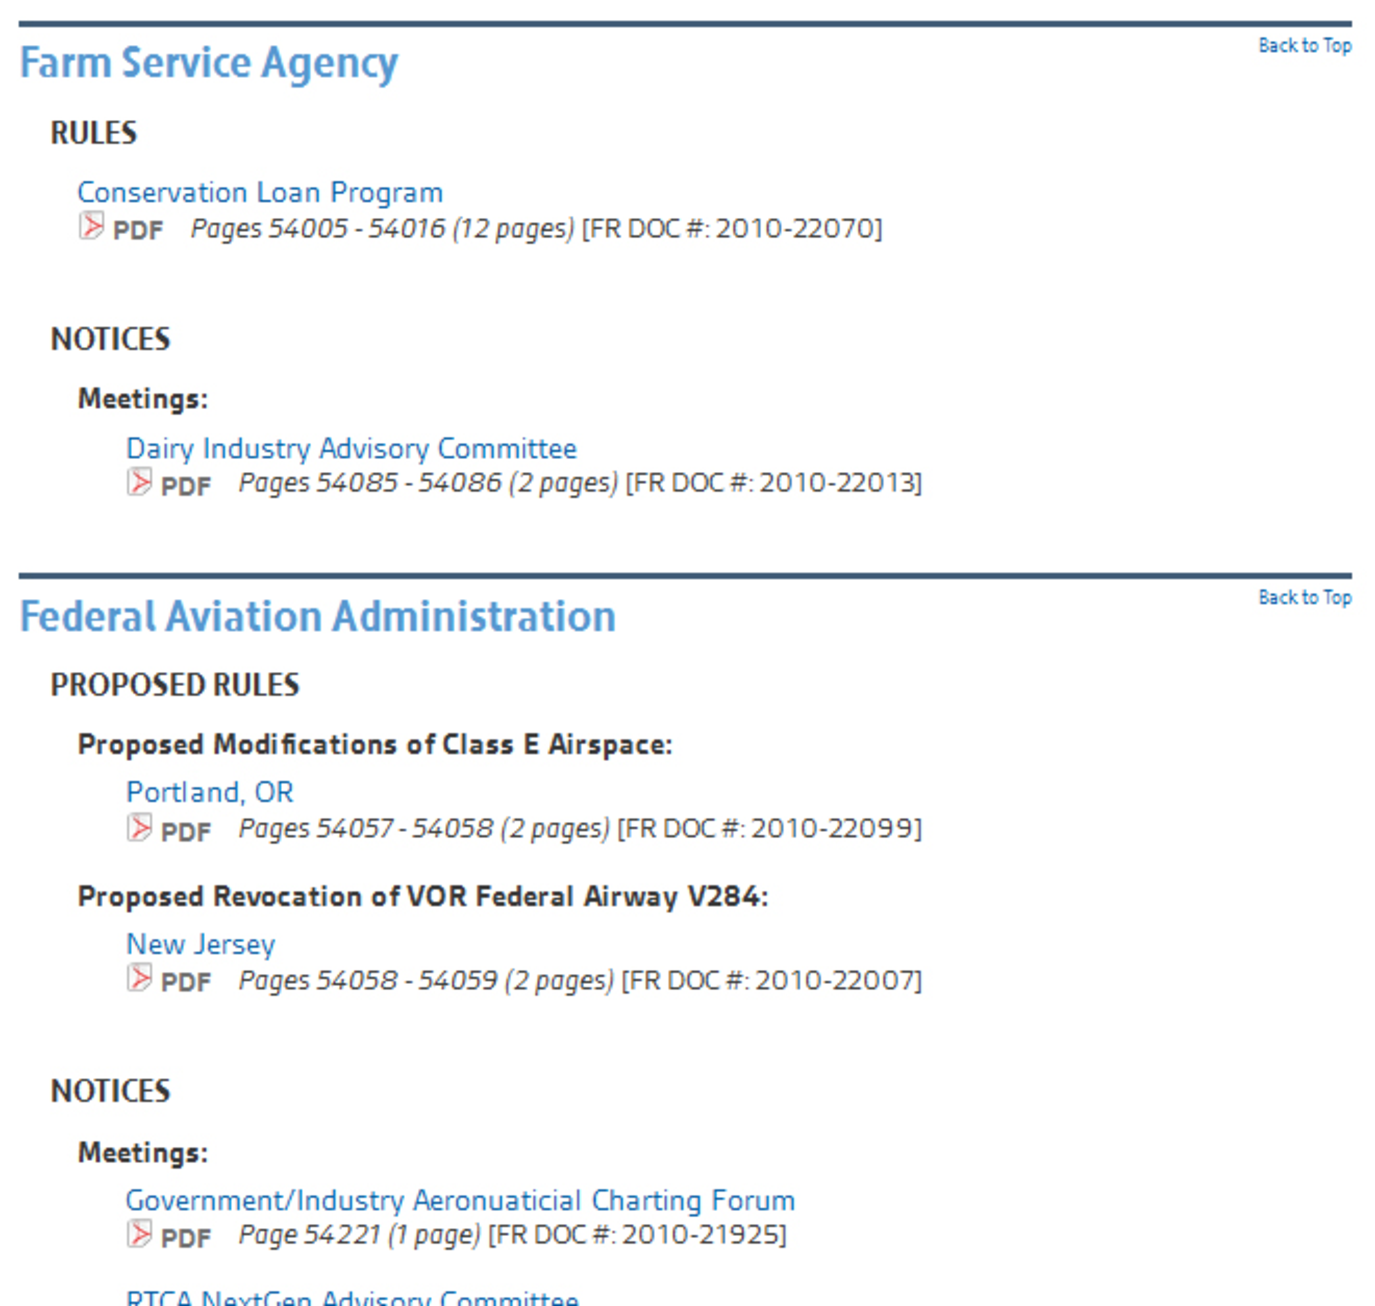
\includegraphics[height=3.25in,width=4in]{3Feb2010.pdf}
\end{figure}
\end{frame}

\begin{frame}[fragile]
\frametitle{Pulled XML Version}
\scriptsize
\begin{verbatim}
     <AGCY>
      <EAR>Farm</EAR>
      <HD>Farm Service Agency</HD>
      <CAT>
        <HD>RULES</HD>
        <DOCENT>
          <DOC>Conservation Loan Program,</DOC>
          <PGS>54005-54016</PGS>
          <FRDOCBP D="11" T="03SER1.sgm">2010-22070</FRDOCBP>
        </DOCENT>
      </CAT>
      <CAT>
        <HD>NOTICES</HD>
        <SJ>Meetings:</SJ>
        <SJDENT>
          <SJDOC>Dairy Industry Advisory Committee,</SJDOC>
          <PGS>54085-54086</PGS>
          <FRDOCBP D="1" T="03SEN1.sgm">2010-22013</FRDOCBP>
        </SJDENT>
      </CAT>
    <AGCY>
      <EAR>FAA</EAR>
      <HD>Federal Aviation Administration</HD>
      <CAT>
        <HD>PROPOSED RULES</HD>
        <SJ>Proposed Modifications of Class E Airspace:</SJ>
        <SJDENT>
  
\end{verbatim}
\end{frame}

\begin{frame}
\frametitle {Things I have or can get}
\begin{itemize} \addtolength{\itemsep}{1\baselineskip}
\item Total # of All appointments
\item Data on New Hires to the Agency, including numbers per agency and titles.
\item Data on People who left or were fired from an Agency
\item Data on rules, notices, etc. agencies are making
\item Names associated with titles for those serving in election years only.
\item An organizational chart of an agency showing where the Schedule C appointee is supposed to serve.
\end{itemize}
\end{frame}

\begin{frame}
\frametitle{Questions for you}
\begin{itemize} \addtolength{\itemsep}{1\baselineskip}
\item How to know whether or not B is doing something if we can't observe it?
\item How to know whether or not B is "just" patronage?
\item What would it take to buy whether or not A's actions are correlated with B's if we can't observe them?
\item What could be interesting or fruitful from these FR data? 
\end{itemize}
\end{frame}

\end{document}
